\chapter{Reference Model}\label{cha:reference}
The \gls{reference model} of the LOGwear project is a model that shows how the communication from a wearable to the \gls{wms} or some other system might work. This does not mean that every communication necessarily needs to be implemented like displayed in the \gls{reference model}, but that in general every wearable is able to communicate with an underlying system in the way it is displayed.
The model can be seen in figure \ref{fig:referenceModel}.
\begin{figure}[htbp]
	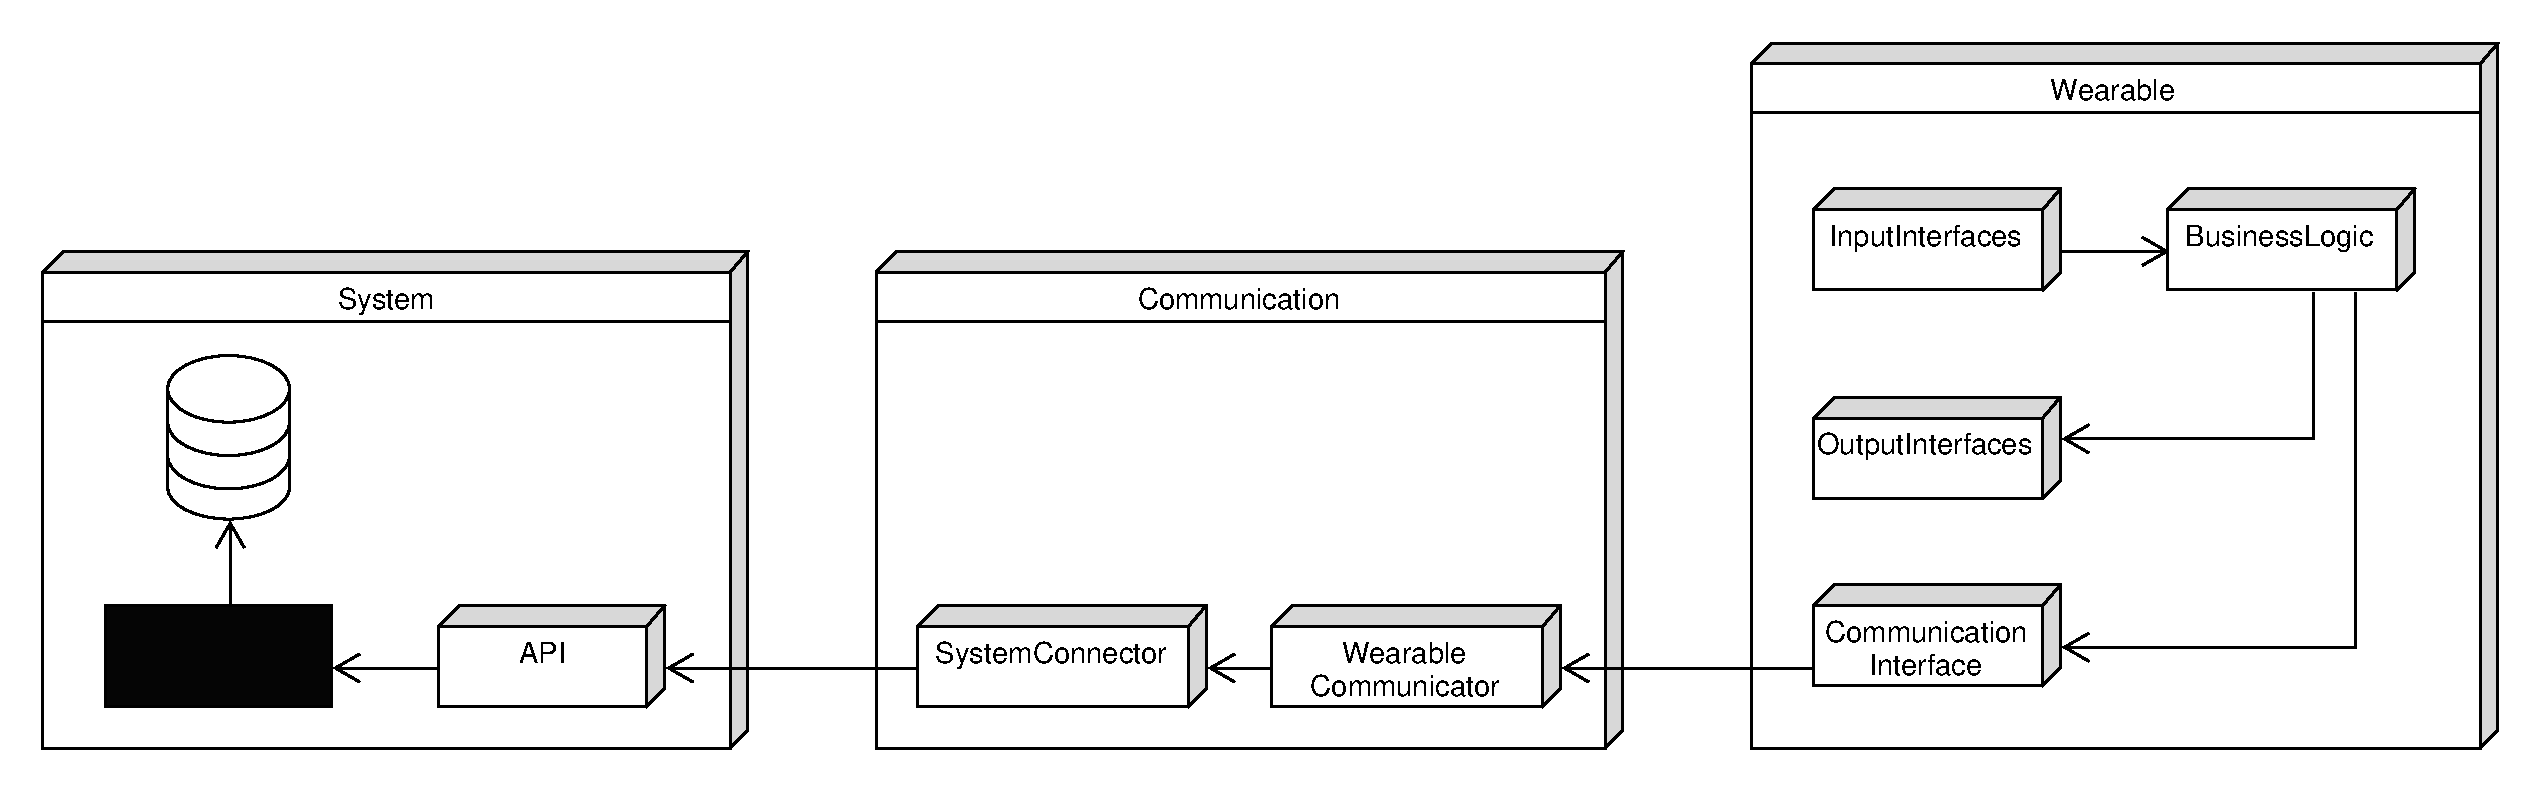
\includegraphics[width=\linewidth]{images/PackageModel_ReferenceArchitecture}
	\caption{Reference Model LOGwear}
	\label{fig:referenceModel}
\end{figure}

\section{Definition}
A \gls{reference model} is an abstract design used to help others understand the general concept and the relationships between existing entities of a specified environment. Furthermore a \gls{reference model}, in general, does not model anything with a specific technology in mind and rather models everything as general as possible. This is done so that when creating an architecture around the \gls{reference model}. The \gls{reference model} can be used as a template to start working with. Not as a constraint, that holds the architects back. When implementing the \gls{reference model} with a specific technology, it is needed to change existing parts or add new parts to fit the given constraints. A \gls{reference model} as is, is not directly implementable due to the abstract nature.

The aim for a \gls{reference model} is to standardize the way how developers in the future implements an application in the given domain, regardless of the used technologies.\citep{website:oasis-rm}

\section{Requirements}
The reference model is an abstract construct, therefore the functional requirements towards it are taken as example to prove the validity of the model. The functional requirements are listed in the form of use cases The non-functional requirements are towards the model itself and not towards an implementation of it. 

\subsection{Functional Requirements}
The functional requirements represents example cases that should be possible to implement with the reference model. The cases that will be given do not need to be fulfilled all at once, but all of them should be possible with the reference model. Given in the following list are short descriptions of the use cases, while the full use cases themselves can be seen in the appendix, section \ref{sec:useCasesReferenceModel}. The example cases given here are based on the demo scenario chosen, but more use cases can be defined for different scenarios.

\begin{description}
	\item[Get Order] \hfill \\
		An order document is fetched and in some way displayed to the worker.
	\item[Order Confirmation] \hfill \\
		The order the worker is currently working on is being worked on and the parts of the order is being confirmed. When all parts of the order are finished the whole order can be confirmed.
	\item[Order Control] \hfill \\	
		When an order is being picked, the wearable is supporting the worker in counting the right number of parcels and picking the correct article in the first place.
\end{description}


\subsection{Non-Functional Requirements}
The non-functional requirements towards the reference model are the most important details that were taken in consideration when the reference model was designed. They can be seen in the following list:

\begin{description}
	\item[Documentation] \hfill \\
		The reference model needs to be properly documented. The advantages and disadvantages of the design need to be properly explained to a person that potentially wants to implement a system based on it.
	\item[Extensibility] \hfill \\
		The reference model needs to be extensible since some companies might have some more requirements towards their system than is intended for a general case. Adding functionality to the reference model should be possible.
	\item[Modifiability] \hfill \\
		The existing ideas of the reference model should be modifiable. Companies are going to use different wearables and infrastructure, and the reference model should be adjustable to fit a lot of possibilities without the need to create a completely new system architecture.
\end{description}

\section{Design}
As can be seen in figure \ref{fig:referenceModel} the \gls{reference model} is divided into three different packages that all fulfil different responsibilities. First it will be described what this \gls{reference model} can help to create. Therefore the general thought behind the whole model will be explained and afterwards the three packages \texttt{system}, \texttt{communication} and \texttt{wearable} will be explained on their own.

The concept is simple, a wearable is connected to a communication layer, that then again connects to a system, that could be anything, as long as it has an \gls{api}. The arrows are not indicating an information flow but rather an instruction flow. The box that the arrow leaves does invoke an instruction in the box that the arrow points to. The sources of information are generally the \texttt{InputInterfaces}, and the incoming information is spread from there. Depending on the incoming information, actions are invoked. 

The \gls{reference model} is purposely minimalistically designed, to allow most infrastructures and wearables, to apply the model, with as few changes as possible. If for example a new \gls{wms} was used the only component that needs to be changed is the \texttt{SystemConnector} in the \texttt{communication} package. In that case, the wearable that are in use, can also continue to work, just like they normally would, without the need for a new version to be deployed on all of them.

\subsection{Wearable}
The \texttt{\gls{wearable}} package is representing the actual physical wearable, or a set of wearables, that a worker is using. This could be either \gls{smartglasses}, \gls{smartwatch}es, a ring-scanner or some other \gls{wearable}. It could also be a combination of wearables that is used in order to fulfil a certain task. In such cases it is still possible to stick to the \gls{reference model} either by changing the existing model, with multiple \texttt{BusinessLogic} classes in the different wearable and a manager that could handle that. Or it could be, that even when using multiple wearables at once, a single wearable is handling the business logic of all wearables. Then the other wearables could be addressed by just their input- and output- interfaces.

Further on the wearable package is again held as simple as possible. The \texttt{InputInterfaces} are there to get information from the outside world and the \texttt{OutputInterfaces} are there to somehow represent information to the outside world. The \texttt{BusinessLogic} is there to process the incoming data and invoke the appropriate actions, that could be either displaying some information to the user or making a call to the underlying system through the \texttt{CommunicationInterface}.

The \texttt{CommuncationInterface} is the means of communication with an outside computer source, this could be radio, bluetooth, \gls{rest} via \gls{wlan} or some other way of communication. The \texttt{WearableCommunicator} in the \texttt{Communication} package just needs to be able to receive and understand the messages.
\subsection{Communication}\label{subsec:communication}
The \texttt{communication} package is existing due to the different technologies used from \gls{wearable}s to connect to other computing devices. The communication layer might also be the only place, where information can be fully controlled by the developer, this is especially interesting when the \texttt{system} is controlled by a third-party. Also needed actions can be taken, if the incoming data has to be transformed into a different format, before either the \texttt{\gls{api}} or the \texttt{wearable} can understand it. 

The \texttt{communication} package could potentially be removed, if the wearable has the needed technology in place to directly connect to the \gls{api} of the given system. But this is in general not recommended, as the communication layer allows the developer to create a more standardized flow of information.

\subsection{System}
The \texttt{system} package here can be something like a \gls{wms} of the company. A system that is mostly a black box with an \gls{api} and a database. Most of the time, the \texttt{system} cannot be changed by the developer, therefore the developer needs to use the possible ways to connect to the given \gls{api}.

\section{Variations}

\textcolor{red}{add infromation on how the model could be changed to implement push messages.
}

\textcolor{red}{Differences in how the business logic could be handled  an what it could do, web app, effectively removing business logic in the wearable}

\section{Problems}
The main problem that occurred during the creation of the \gls{reference model} was a problem in communication, regarding the names of \gls{reference model} and \gls{reference architecture}. The initial task was understood to create a general-purpose \gls{reference architecture}, that would connect a \gls{wearable} to some kind of system. During the process of creating the different diagrams for the reference architecture and trying to validate them using code. The problem became obvious that trying to go deeper than the now given \gls{reference model}, as seen in figure \ref{fig:referenceModel}, was impossible to do for a general-purpose implementation.

This is the case because of the nature of the given problem. Being able to use any wearable with any system, for any task. Given that two wearables might have completely different sets of input- and outputinterfaces those could not be defined. The communication interface could be different, which leads to being unable to define a communication standard, while the possibility of any task gives no single action that will always be the same.